\documentclass[11pt,harvard]{article}
\usepackage[letterpaper,top=1in, bottom=1in, left=1in, right=1in]{geometry}
\usepackage{graphicx}
\usepackage[sort]{natbib}
\usepackage{amssymb}
\usepackage{amsmath}
\usepackage{setspace}
\usepackage{url}
\usepackage{pdflscape}
\usepackage{longtable}
\usepackage{threeparttable, booktabs}
\usepackage[export]{adjustbox}
\usepackage{enumitem}
\usepackage{comment}
\usepackage{subcaption}
\usepackage{lmodern}
\usepackage[T1]{fontenc}
\usepackage{setspace} % Load the setspace package
\usepackage{parskip} % Load the parskip package
\usepackage{float}
\usepackage{subcaption}
\usepackage{hyperref}
\usepackage[table,xcdraw]{xcolor}


\author{rCARI study team}
\date{\today}
\title{Sampling Frame for the rCARI Validation Study} 


\begin{document}
	\maketitle \vspace{-2cm}
	\onehalfspacing
	\pagebreak
	\setlength{\parskip}{8pt} % Set the desired space before and after paragraphs
	
% -------	
\section{Background}

The rCARI validation study is a global research project commissioned by WFP and funded by the BHA to investigate and compare remote and face-to-face (F2F) modules of the consolidated approach for reporting food insecurity (CARI). 
The overall goal of the study is to understand to what extent food insecurity reported by rCARI is comparable or compatible with the standard CARI. Both phone (remote) and face-to-face (F2F) data collection modules \& methodologies for collecting food insecurity will used in the study. 

This document outlines the study methodology for the rCARI validation study, specifically sampling process adjusted for country specific context.

The study is designed and implemented as a survey experiment with stratified sample. The following considerations underpin the study areas and final sample selection.

\begin{itemize}[left=2.0em]
	\item Phone ownership \& accessibility within the pilot country
	\item Distribution of food insecurity
	\item Areas of accessibility within the pilot countries
	\item Project budget
\end{itemize}  

\section{Sampling design \& frame}

It is important to emphasize that the purpose of data collection for this study is not to produce population-level estimates but rather to compare the two methodologies with the same comparable population. While it is desirable to collect data from a variety of livelihood zones both urban and rural communities to assess the impact of these differences with respect to modality, national coverage is not the primary objective of this current study. 

Figure 1 below presents the generic study sampling procedure. As mention earlier, selection and inclusion of study area followed a 3-point criterium: i.e., 1) phone coverage, 2) accessibility, and 3) food security situation. Phone coverage is important consideration allowing for equal probability of reaching equal number of households for both remote and F2F interviews, while field accessibility ensures that enumerators can successfully access and interview households in face-to-face. The food security consideration would ensure that at least areas that have different AFI (acute food insecurity) situations are adequately represented in the study sample.

In all 3 pilot countries thus far, the same methodology has been used to identify and select the study areas.  

\begin{figure}[H]
	\begin{center}
		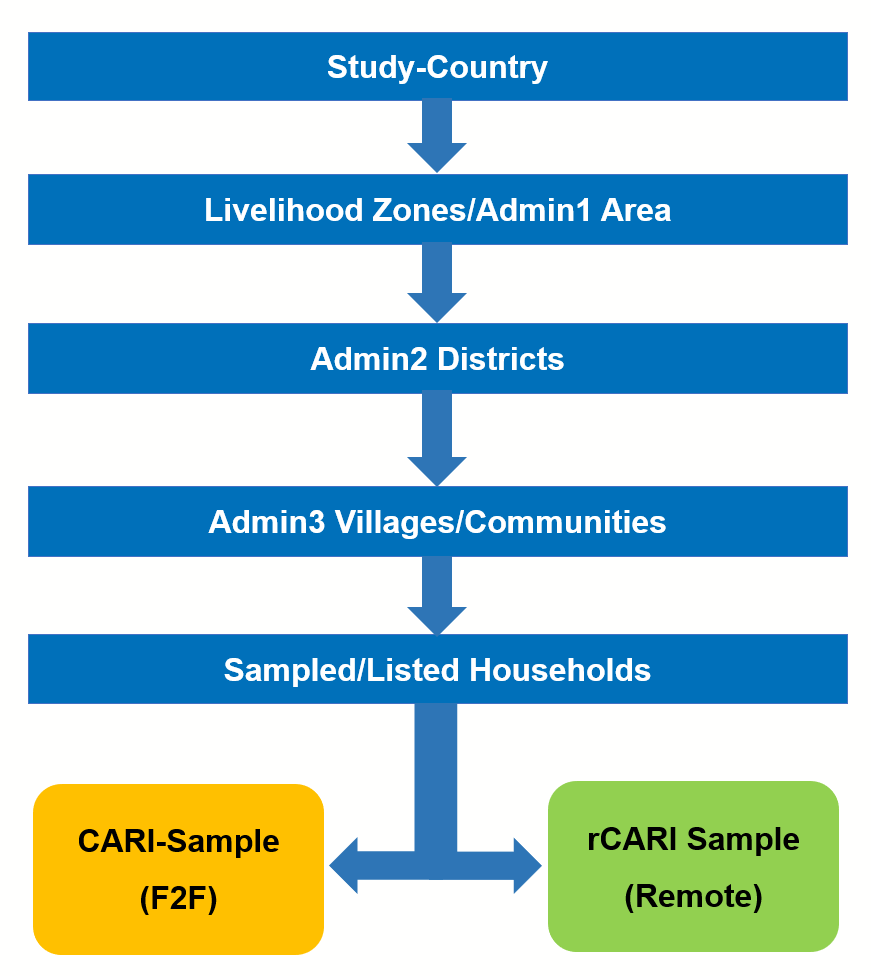
\includegraphics[scale=.5]{2_figure/Sample_Frame.png}
	\end{center}
	\label{fig:Sample_Frame}
	\caption{Sampling and Randomization Procedure}
\end{figure}

The main steps followed in identifying and selecting the admin areas at the various stages are listed and explained below.

\subsection*{Step 1 - Selection of ADMIN1 (Livelihood Zones)}
	In the first stage purposive selection of 2 Admin1 or livelihood areas is done. This will be done collaboratively with the CO and based on phone coverage, food security situation and accessibility. If more than 2 Admin1 Areas meet the inclusion criteria, a list of the potential areas will be compiled and a simple random approach followed to select 2.
	
\subsection*{Step 2 - Selection of ADMIN2}
	In the second stage, 4 ADMIN2 areas will be sampled randomly (2 per ADMIN1 Area based on the outcome of Step 1) from the two ADMIN1 areas that have been selected in the first step.
	
\subsection*{Step 3 - Selection of ADMIN5 (Lowest Admin Areas i.e., villages, communities, or camps)}
	The next step in the process is to compile a list of all the lowest admin areas (ADMIN5 areas) in the selected ADMIN2 areas. The list of ADMIN5s will serve as the primary sampling units (PSUs). A minimum of 20 PSUs (or 25 based on the CO recommendation) will be randomly selected (distributed equally across the two ADMIN1s selected in Step 1). The study sample (households) will be selected from these 20/25 PSUs.
	
\subsection*{Step 4 - Sampling study participants (households (HHs))}
	The final stage of the sampling procedure will be to compile a list of potential households for the study. The sampling frame for the study will be all households in each of 20/25 selected PSUs.
	 
	Household list will be compiled through listing. The listing process will done through a simple random process using the standard random-walk approach (in the absence of any recent household census). The aim is to collect information from households that are as accurate and representative as possible in each study area. Thus, the idea is to give fairly equal chance of selection to all households in each PSU as much as practicable. The study will therefore enlist an equal of number of households, a minimum of 100 households per each PSU taking into consideration attrition from previous studies. 
	
	Trained and conscientious enumerators shall be used for the systematic selection of households. A sampling interval of selecting every 3rd house in the sequence shall be followed. 
	
	To ensure the integrity and ethics of the study, informed consent will be taken from all households during listing phase to ensure that all households understand the survey before being included in the study sample. Based on the number of PSUs selected per country, between 2500-3500HHs will be listed for and used for the randomization process.
	
\subsection*{Step 5 - Randomization of household (HHs)}
	Consented final sampled households in Step 4 are randomly assigned into one of two survey modalities/groups; F2F (CARI group) and Remote (rCARI group). The design is such that the sample will be divided equally between the two groups using a standardized randomization process. 
	
	All interviews (both F2F \& remote) will be conducted simultaneously over the same time frame to ensure that households are reporting food security situation over the same window and also affected by similar geographical situations.
	
% -------	
\pagebreak
% -------	

\subsection{Myanmar}
In Myanmar, the study was implemented amongst IDPs (internally displaced persons) in two regions: Kachin and Shan (Admin 1). The sampling list was compiled using beneficiaries made up of IDPs in the two regions. A total of 20 camps were selected randomly as the primary sampling units (PSU). All households in the selected camps formed the sampling frame for the study in Myanmar. A minimum of 100 households were then randomly selected from each camp for the study (However, because some of the camps had fewer than 100 households, the final sampled households were 1665 in total).

% -------	
\pagebreak
% -------	
\subsection{Ecuador}
In Ecuador, the study was implemented in three regions: Amazonia, Costa and Sierra (Admin1 areas). In addition to the standard selection criteria based on accessibility and food security prevalence, consideration was also given to the safety of the team, considering the political situation at the time of implementing the study.  

A total of 27 Admin5 areas (villages) were randomly selected from the 3 Admin1 areas based on the foregoing criteria. These formed the PSUs for the study in Ecuador. All households in the selected 27 PSUs formed the selection frame and were eligible to be enlisted into the study. A total of 3220 households were listed (approximately 120 households per PSU were randomly selected) for the study in two phases.    

\begin{figure}[H]
	\begin{center}
		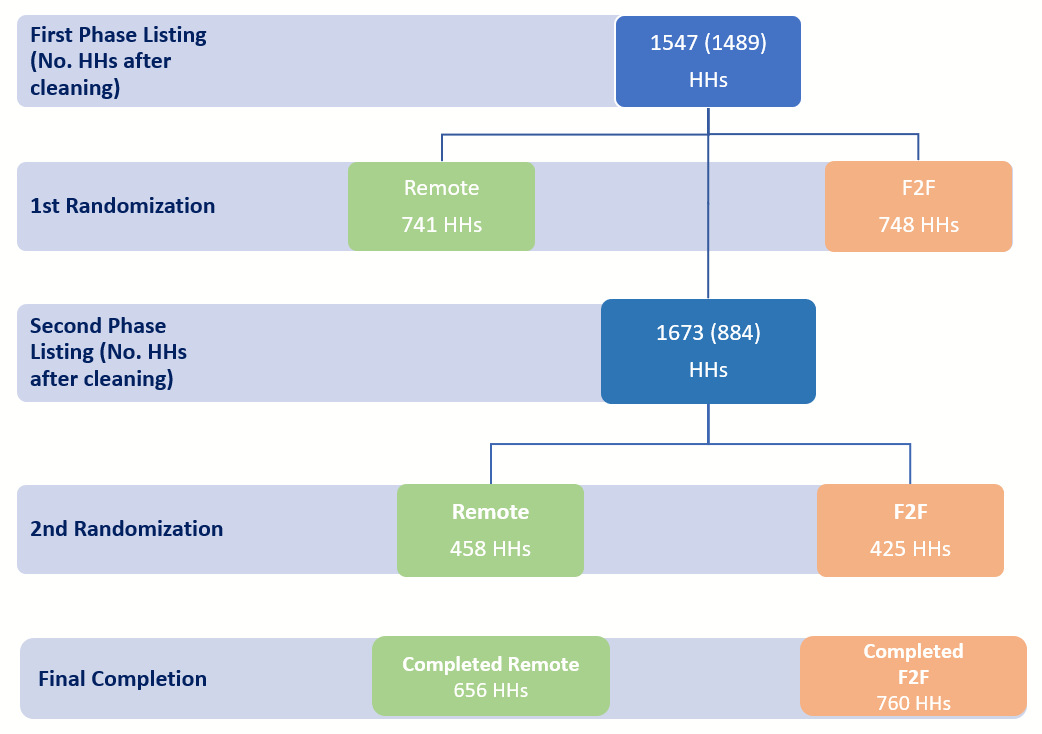
\includegraphics[scale=.65]{2_figure/Ecuador_Sample_Composition.png}
	\end{center}
	\caption{Sampling and randomization in Ecuador }
	\label{fig:Ecuador_Sample_Composition}
\end{figure}

% -------	
\pagebreak
%---------

\subsection{Central African Republic (CAR)}

Study in CAR was implemented in two Prefectures: Mbomou and Nana-Gribizi (he two most accessible areas (aside from Bangui) that also had a varying level of food security).  

The selection of PSUs followed a similar pattern using field access (security situation) and mobile phone network coverage. The list of Admin5 areas that met the access and mobile phone coverage criteria formed the sampling frame. A total of 25 Admin5 areas (villages) were randomly selected from the list of Admin5 areas compiled jointly be the CAR CO and the local mobile phone service providers (to ensure that all Admin5 areas selected had mobile phone network). Admin5 areas without phone coverage were automatically excluded. 

To ensure that the final sample was a mix of rural and urban households (taking into consideration there was a potentially different food security situation between rural and urban households), sub layer of locality was included during the selection of Admin5 areas so that the final sampled PSUs were a combination rural and urban areas. 

The sampling frame for the study was all households in the 25 selected ADMIN5 areas. The listing phase was conducted through the random-walk methodology in each selected PSU by trained enumerators. A minimum of 100 households/respondents per PSU totalling 2500 households/respondents were listed as potential study participants. Phone numbers of the main respondent and any other phone numbers within the household that could have been used to contact the main respondent during the survey were collected. Drawing from the data collection experience in Myanmar and Ecuador, a number of demographic characteristics such as age of household head, gender of household head, household size, and ownership of common household assets was collected during household listing and used for the statistical balance test. 

\begin{figure}[H]
	\begin{center}
		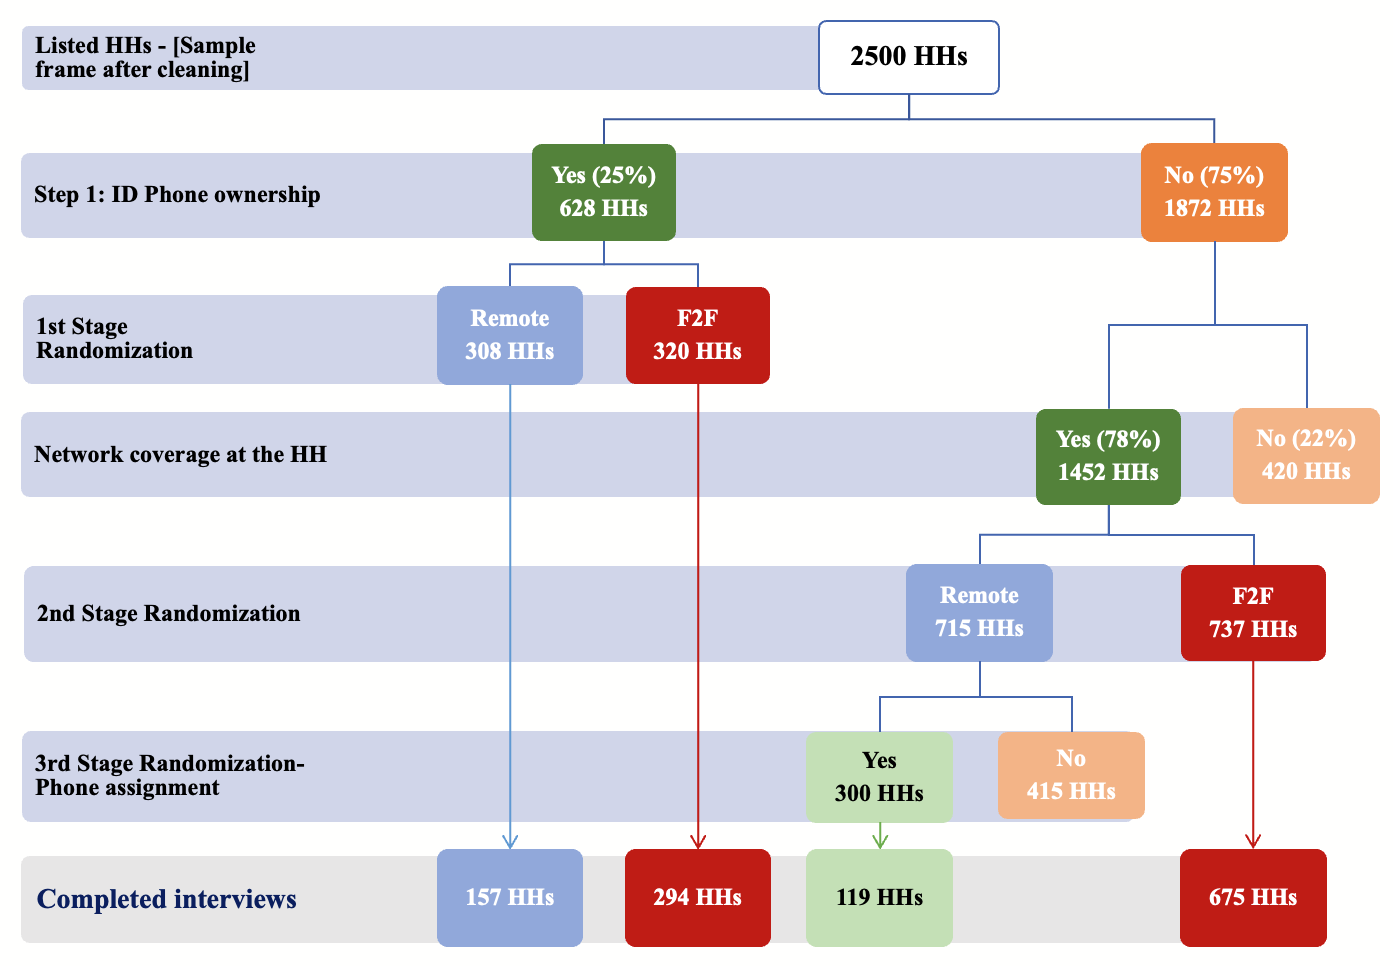
\includegraphics[scale=.3]{2_figure/CAR_Sample_Composition.png}
	\end{center}
	\label{fig:CAR_Sample_Composition}
	\caption{Sample Composition and Completion in CAR}
\end{figure}

\pagebreak
% -------	
\subsection{Burkina Faso}

Following in the study framework illustrated in Figure 1, the first three steps have already been completed. In conjunction with the Burkina Faso CO, two prefectures (ADMIN1s) namely: Centro and North prefectures have been selected to be the study areas (selection based on accessibility and phone coverage). 

Based on the list of ADMIN5 areas available to the CO, an initial list of 25 villages (Admin 5 areas) have been randomly selected to form the main PSUs from which the participating households would be selected following a random walk procedure. 

The household sampling frame will be made up of all households in each of the selected 25 PSUs. Households would be enlisted into the study through a household listing process that would be implemented through a random walk across each PSU. Prior to the selection process, carefully selected, trained and conscientious enumerators will be engaged for the selection and listing process in each PSU. Starting from a known point, enumerators will identify and enlist systematically every 3rd household and with their consent be included in the study sample.

During the listing phase, once the household head agree to participate in the study, a standardized listing questionnaire to collect basic household and respondent characteristics such as age, gender of household head, education of household head, mobile phone ownership, household size, ownership of some basic assets, housing, (WASH) etc. ( these are to be used later for the purpose of randomization) will be administered. 

Listed households that do not have access to mobile phones within the household or phone coverage will be dropped during the randomization. Similarly, households with incomplete baseline and contact information will be dropped from the final. 

The following Administrative areas have been selected (employing both purposive and random methods) as the study areas. Admin1 areas were purposively sampled based on these regions meeting the inclusion criteria of accessibility, security and phone network coverage. 

The selection of the ADMIN5 areas followed a simple random sampling procedure drawing random 25 villages from the census of all villages from the 2 ADMIN1 areas. The selected admin areas are listed below.

\subsection*{ADMIN1 AREAS (2)}
\begin{itemize}[left=2.0em]
	\item[1.]North Prefecture, and
	\item[2.]Centro Prefecture
\end{itemize}

\subsection*{ADMIN3 AREAS (4)}
Two each have been sampled from the North and Centro prefectures respectively.

\begin{itemize}[left=2.0em]
	\item[1.]Boulsa
	\item[2.]Guibare
	\item[3.]La-Todin
	\item[4.]Oula
\end{itemize}

\subsection*{ADMIN5 AREAS (20)}
The Admin5 areas selected were even distributed across the Admin1 \& 3 areas respectively. In total 10 Admin5 areas have been selected from each Admin1 area.

\begin{itemize}[left=2.0em]
	\item[1.]Secteur 6
	\item[2.]Kiendsom
	\item[3.]Secteur 5
	\item[4.]Nièga
	\item[5.]Kobouré
	\item[6.]Barsa
	\item[7.]Yilou
	\item[8.]Vousnango
	\item[9.]Wattinoma
	\item[10.]Sakoudi
	\item[11.]Minissia
	\item[12.]Gogho
	\item[13.]Pendogo
	\item[14.]Ramessoum
	\item[15.]Lâ-Todin
	\item[16.]Bourbo
	\item[17.]Reka
	\item[18.]Bouro
	\item[19.]Tilli
	\item[20.]Ouro Mossi 
\end{itemize}


\subsection*{The Questionnaire}


\end{document}
